\section{Load Testing Plan}
\label{se:test_plan}

In \cref{subse:modules_weather_data_integration_sys} \hl{we discussed three modules of a weather data system such as integration, assimilation, and dissemination. Each of those modules is mapped and handled in the WDIAS as below.}
\begin{enumerate}
    \item \emph{Import} modules (integration modules)
    \item \emph{Export} modules (Dissemination modules)
    \item \emph{Extension} modules (Assimilation modules)
\end{enumerate}
Other than above, \emph{adapter modules} act as the core modules and the base of the system. Also, query modules allow the users to query for the timeseries based on the metadata and enable performing Geo-based queries based on the locations.

The test plan is to perform the load test on each above module as a separate entity to analyze the individual module scalability.
Then perform load testing on the whole system, and analyze the scalability in the system. Two variables can vary while doing performance testing.
\begin{enumerate}
    \item Number of requests made to the system at a given time (\acrfull{rps})
    \item Request size
\end{enumerate}
A timeseries is a series of data points in time order. The system may receive the data points in multiple requests.
The request size can vary based on the use case from one data point to multiple data points. As few examples;
\begin{itemize}
    \item A weather station may send the current water level in a regular period of 1 minute. In such a case, it always comes as a request with one data point with higher frequency.
    \item Due to resource issue such as batteries, a weather station can collect data points for a given period and send as a batch. Another example would be,
A weather station can collect the precipitation at each 5 minute period and send all the data in 1-hour intervals.
    \item The forecast precipitation data from the \acrshort{wrf} model can be extracted for a day in a one-hour interval and store in the system.
\end{itemize}

The percentage of each data type can be varied depending on the situation. But most of the applications collect much data from the weather stations to correct and validate the models' data. These weather stations can send the data in different frequencies with different parameters such as precipitation, temperature, humidity, wind direction, etc. Most of these are scalar data. Parameters such as wind direct are vector data which has less percentage compared to scalar data. On the other side, most of the grid data generate from models and simulations. Those produce in less frequency due to the cost of the computer resource to produce results. After considering those factor we came up with 70\% scalar, 20\% vector, and 10\% grid values.
%\begin{itemize}
%    \item Scalar - 70\%
%    \item Vector - 20\%
%    \item Grid - 10\%
%\end{itemize}

As an upper limit of such scenarios while designing the performance testing, it uses the following;
\begin{itemize}
    \item Hourly (24 data points) 
    \item Every 30 minutes (48 data points)
    \item Every 15 minutes (96 data points) - One request is equivalent to a data points send by a weather station in 15 minutes interval for a single day
\end{itemize}

\begin{figure}[htp]
    \centering
    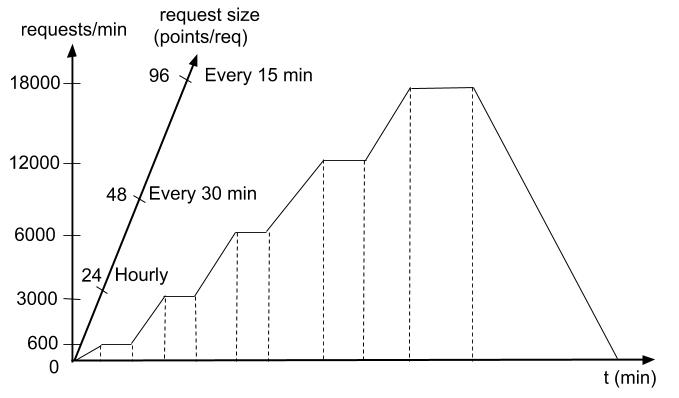
\includegraphics[width=0.8\textwidth]{results/work_load/performance_study_v4.jpg}
    \caption{\acrshort{wdias} load testing plan with changing the request size and \acrshort{rps}}
    \label{fi:performance_study_load}
\end{figure}

\cref{fi:performance_study_load} shows the summary of this section, load testing plan with changing the request size and perform load testing with increasing the \acrshort{rps} over time. As shown in the figure, for a given request size the \acrshort{rps} increased in steps. In each step, the \acrshort{rps} holds for a moment to give some time for the system to get stabilized. Thus at each milestone, we can measure the performance of the system and study the stability of the system. After it comes to the peak time, the \acrshort{rps} holds for more time than the previous milestones. During the \acrshort{wdias} load testing, we are planning to have a peak of 18,000 requests per minute. Holding the peak load will help to show whether the system is capable of scaling more than the proposed load testing plan. After the peak, the test case goes through a cool-down period to measure the ability to shrink down the resources when there is not any load on the system.

%%%%%%%%%%%%%%%%%%%%%%%%%%%%%%%%%%%%%%%%%%%%%%%%%%%%%%%%%%%%%%%%%%%%%%%%%%%%%%%%
\subsection{\hl{Test Scenarios}}
\label{subse:test_plan_flow}
Following are the test cases which are planned to performance test cases;
\begin{enumerate}
    \item Test Setup to create timeseries in 1hr, 30min and 15min intervals and create metadata of the timeseries
    % \item Extensions
    % \begin{itemize}
    %     \item Create Extensions for /Aggregation\_Accumulative, /Interpolation Linear, /Validation Missing Values (OnChange and OnTime)
    %     \item Plan for the 15 minutes of test run with the request size of 15min data. (total 0.25 hours)
    %     \item Do with Import Timeseries with error data which will go through extensions.
    % \end{itemize}
    \item Import + Extension + Export + Timeseries Queries
    \begin{itemize}
        \item Plan for 30 minutes of the test run with the request size of 1hr (60min) data.
        \item Plan for 30 minutes of the test run with the request size of 30min data.
        \item Plan for 30 minutes of the test run with the request size of 15min data.
        \item Plan for 30 minutes of the test run with the request size of 15min data with auto-scaling.
        \item All test plan run against 60min, 30min and 15min request size of data. Another test plan runs with enabling the auto-scaling. (total of 2 hours)
    \end{itemize}
    \item Query
    \begin{itemize}
        \item Query Timeseries
        \item Plan for the 5 minutes of test run. (total 1/12 hours)
    \end{itemize}
\end{enumerate}


%%%%%%%%%%%%%%%%%%%%%%%%%%%%%%%%%%%%%%%%%%%%%%%%%%%%%%%%%%%%%%%%%%%%%%%%%%%%%%%%
\subsection{Performance Metrics}% of Load Testing}
\label{subse:test_plan_metrics}
During the performance analysis, the following metrics are used to measure the performance of the system.
\begin{itemize}
    \item \emph{Throughput} -- Number of requests that can processed per unit time. Normally for \acrshort{wdias} performance observations, it uses \acrfull{rps} to measure the throughput.
    \item \emph{Latency} -- Time is taken to respond to the sent request to the system. Normally it measures with milliseconds (ms) in the \acrshort{wdias}. During the performance analysis, it measures the minimum response time, maximum response time, the average response time, and standard deviation. The standard deviation measures the mean distance of the values to their average.It gives an idea of the dispersion or variability of the measures to their mean value. So, if the deviation value is low compared to the mean value, it will indicate that the measures are not dispersed (or mostly close to the mean value) and that the mean value is significant. Other than that, it measures the response time into 90\% percentile, while gives the best response time up to 90\% percent of the responses.
    \item \emph{Resource utilization} -- Resource Utilization is calculated based on the CPU and Memory usage via the \acrshort{k8s} metrics server. It calculates the resource utilization over 60 seconds time window. Network usage is getting based on the actual physical machines.
    \item \emph{Auto-scaling} -- The \acrshort{wdias} is running with two configurations. First is, since it is running the microservice as docker containers, it allows to increase or shrink the resource usage and share the resources within a physical machine. Second is, running with auto-scaling enabled for the microservice which are using higher resources.
\end{itemize}
